\documentclass[class=book, crop=false, oneside, 12pt]{standalone}
\usepackage{standalone}
\usepackage{../../style}
\usepackage[normalem]{ulem}
\graphicspath{{./assets/images/}}

% arara: pdflatex: { synctex: yes, shell: yes }
% arara: latexmk: { clean: partial }
\begin{document}
\part{Aftermath}
\chapter{Conclusioni}
In questo capitolo conclusivo rivedremo velocemente le fasi del  processo di compilazione dando una spiegazione generale e complessiva di tutto quello he abbiamo approfondito nei capitoli precedenti; dove si presenterà l'occasione andreamo anche ad inserire dei commenti interessanti che a suo tempo non abbiamo menzionato per non appesantire eccessivamente la trattazione teorica.

Partiamo quindi con il ripetere, per l'ennessima volta, in maniera schematica le fasi della compilazione ed il loro scopo:
\paragraph{Analisi lessicale} In questa fase si prende la stringa in ingresso e la si trasforma in una sequenza di token, che diamo in pasto all'analizzatore sintattico.

\paragraph{Analisi sintattica} A questo punto verifichiamo se la sequenza di token aderisce alla specifica grammatica del linguaggio di programmazione che stiamo utilizzando, se è così ricaviamo un albero di parsing per la stringa data in input. 

\paragraph{Analisi semantica} Qui vengono considerate caratteristiche del linguaggio che non possono essere descritte agilmente dalla grammatica, si va a valorizzare e ad assegnare attributi a tutti gli elementi riconosciuti nelle fasi precedenti.
	
\paragraph{Generazione del codice intermedio} In questa fase si genera appunto una rappresentazione intermedia della stringa data in input e si va a compiere possibili ottimizzazioni (molte delle quali indipendenti dal llinguaggio finale, tatget code).

\paragraph{Generazione del codice macchina}	A questo punto si traduce il codice intermedio in linguaggio macchina ed eventualmente si inseriscono ulteriori ottizzazioni legate al particolare linguaggio macchina.
    
Noi abbiamo visto tutte queste fasi separatamente, ma ricordiamo che spesso e volentieri vengono eseguite in simultanea per ottimizzare i tempi.
È arrivato il momento di rispettare le tradizioni, quindi ora introdurremo un esempio che ci permetterà di andare a rianalizzare più approfonditamente tutte le fasi della compilazione.
\section{Analisi lessicale}
\begin{equation}
    \label{eq:last-ex}
    position = initial + rate * 60
\end{equation}
Data la stringa in input rappresentata in \ref{eq:last-ex} l'analizzatore lessicale va a ricavare i token e ad inserire tutte le informazioni che ricava nella symbol table, ottenendo un risultato come quello che si può osservare in seguito.
Riportiamo la lista di identificatori.
\begin{equation}
    \label{eq:last-ex-tokens}
    <id,1> assign <id,2> sumop <id, 3> mulop <num, 60>
\end{equation}
Riportiamo ora la tabella dei simboli (Tab.\ref{tab:last-ex-symbol-table}).
\begin{table}[H]
	\centering
	\subimport{assets/tables/}{symbol-table.tex}
    \caption{Symbol table ricavata dall'analisi lessicale}
    \label{tab:last-ex-symbol-table}
\end{table} 

In questo caso specifico l'analizzatore lessicale va a riconoscere \(position\), \(initial\) e \(rate\) come identificatori (nota che nella lista di tokens, Eq.\ref{eq:last-ex-tokens}, sono inseriti il link agli identificatori); allo stesso modo l'analizzatore lessicale va a riconoscere gli operatori che vengono utilizzati ed infine riconosce il numero e crea un token che specifica che è un numero e ne contiene il valore.

La stringa che andremo ad analizzare nell'analisi sintattica si dimenticherà poi dei riferimenti agli identificatori, delle parentesi angolari e dei valori numerici, quindi sostanzialmente andrà ad analizzare la stringa:
\begin{equation}
    id = id + id * num
\end{equation}
L'analizzatore lessicale deve riconoscere le parole chiave del linguaggio e deve anche disambiguarle da eventuali identificatori ambigui (ad esempio \(while22\)); per questa ragione gli analizzatori lessicali utilizzano automi a stati finiti, sia in versione deterministica che non deterministica.
In qualsiasi caso i tipi di linguaggi che gli analizzatori lessicali vanno ad approcciare sono tutti linguaggi regolari derivati da grammatiche regolari.

Di questa fase, durante il nostro percorso, abbiamo visto tutti i passaggi: abbiamo ricavato l'automa per l'analisi lessicale da una determinata grammatica, poi abbiamo visto come minimizzaretale automa ed infine il suo utilizzo per riconoscere un linguaggio regolare.
Ora possiamo quindi passare all'analizzatore sintattico la lista di token che abbiamo ricavato e gustarci il prossimo flashback. 

\section{Analisi sintattica}
Nella fase di analisi sintattica vogliamo innanzitutto capire se la lista di token in ingresso aderisce alle regole della grammatica;da tale lista si ottiene, nel caso la stringa sia corretta, un albero di derivazione.
Nel nostro esempio quello che andiamo ad ottenere dalla lista di token in Eq.\ref{eq:last-ex-tokens} è il seguente albero di parsing.
\begin{figure}[H]
    \centering
    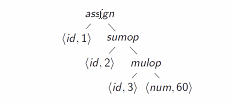
\includegraphics[width=.4\textwidth]{final-example-parsing-tree.png}
    \caption{Parsing tree ricavato dal nostro esempio}
    \label{fig:last-ex-parse-tree}
\end{figure}
Per l'analisi sintattica noi abbiamo studiato ed utilizzato le due famiglie principali di metodi di parsing (ovvero leftmost e rightmost). 
È da notare però che esistono parser adatti all'analisi di una qualsiasi grammatica libera, tuttavia questi hanno complessità minima \(n^3\) il che li esclude dalla nostra wishlist.
I parser che abbiamo affrontato in questo testo riescono a ricavare un albero di derivazione con complessità LINEAREH.

Abbiamo visto due tipologie principali di parsing:
\begin{itemize}
    \item parsing top-down;
    \item parsing bottom-up.
\end{itemize} 

\subsection{Parsing top-down\\ \small{Quello bello}}
Quando ci troviamo al cospetto di grammatiche LL(1) riusciamo a ricavare il parse tree senza bisogno di backtrack utilizzando il parsing top-down.
La strategia di analisi del parsing top-down prevede di partire dalla derivazione dello start symbol e poi utilizzando la derivazione di tipo leftmost andare a costruire il parse tree.
Se la grammatica è LL(1) va tutto liscio ed otteniamo l'albero di parsing in men che non si dica, se non lo è dobbiamo ricorrere al backtrack, ma noi non vogliamo che questo succeda, Larry.

Abbiamo quindi visto delle caratteristiche che vogliamo evitare per assicurarci di lavorare sempre con grammatiche LL1:
	- Le grammatiche ricorsive sinistre non sono LL1, ma abbiamo visto come trasformarle
	- Le grammatiche fattorizzabili a sinistra non sono ll1, ma come prima abbiamo visto come eliminare questo problema
	- Le grammatiche ambigue non sono LL1, perché esiste almeno una stringa nel linguaggio che può essere derivata in 2 modi diversi (sempre leftmost)

L'altra grossa famigliola di grammatiche che abbiamo visto sono quelle che possono essere analizzate in maniera bottom-up, abbiamo visto grammatiche:
	- SLR
	- LR1
	- LALR
Il goal dell'analisi bottom-up è sempre lo stesso, ma il modo in cui si va a ricostruire l'albero di derivazione è opposto al top-down, si parte dalle foglie e si va alla radice.
Indifferentemente dal tipo di grammatica che stiamo analizzando il modo per ricavare il parse tree è sempre l'utilizzo dell'algoritmo shift-reduce una volta che si ottiene la parsing taable per quel tipo particolare di grammatica.

Mentre eseguiamo shift reduce andiamo ad analizzare la stringa carattere per carattere ed usando la parsing table come mappa ci spostiamo nel buffer di lettura (mosse di shift) e quando incontriamo una stringa che può derivare da una certa produzione della grammatica andiamo ad effettuare una mossa di reduce.

Le 3 grammatiche che abbiamo visto per il parsing bottom-up si differenziano per quanto sono fini le condizioni per riconoscere quando inserire una mossa di riduzione.
Quello che succede però è che utilizzando grammatiche e parsing SLR otteniamo un automa per il parsing semplice ma povero di informazioni, mentre LR1 ci fornisce degli automi molto più precisi, con dei lookahead set che ci danno molte più informazioni su quando applicare le riduazione (grazie ai lookahead set).

Poi ci sono le grammatiche LALR che si trovano tra SLR e LR1, ci offrono una tabella di parsing delle dimensioni di una tabella SLR ma hanno una complessità di calcolo leggermente superiore alle grammatiche LR1.

\end{document}
